\documentclass[a4paper]{article}
\usepackage[utf8]{inputenc}
\usepackage{geometry}
\usepackage{fancyhdr}
\usepackage{imakeidx}
\usepackage{titlesec}
\usepackage{lipsum}
\usepackage{graphicx}
\usepackage{float}
\usepackage{tocloft}

\renewcommand{\contentsname}{Indice}

\geometry{left=2.5cm, right=2.5cm,bottom = 3.6cm}
\setlength{\topmargin}{-1.5in}
\pagenumbering{arabic}



\title{Corso Di Laurea In Informatica}

\date{}

\begin{document}

\maketitle

\begin{center}
\vspace{3cm}
\Huge{\textbf{Elaborazione di Segnali ed Immagini}}
\end{center}

\begin{center}
\vspace{3cm}
\Huge{\textbf{Progetto: Percorso N° 1}}
\end{center}

\begin{center}
\vspace{1cm}
\huge{\textmd{Analisi di difetti di tessiture}}
\end{center}

\begin{center}
\vspace{2.5cm}
\begin{tabular}{ll}
\vspace{0.5cm}
\huge{\textmd{Simone Brunello: VR437366 }} \\ 
\vspace{0.5cm}
\huge{\textmd{Francesco Ridolfi:  VR437081}} \\

\huge{\textmd{Elisa De Rossi: VR429665 }}
\end{tabular}
\end{center}

\footskip = 200.pt

\clearpage
\null
\clearpage

\newpage
\topskip = 50.pt
\renewcommand{\cftsecfont}{\Large\scshape}

\tableofcontents{}
\addtocontents{toc}{~\hfill\textbf{Page}\par}
\newpage


\titleformat*{\section}{\Huge{}\bfseries}

\newpage
\topskip = 50.pt

\section{Introduzione}
\setlength{\baselineskip}{0.8cm}
{\vspace{0.5cm}\fontsize{6mm}{6mm}\selectfont In questo elaborato si deve modificare ed ampliare lo script Matlab fornito durante le lezioni di laboratorio in modo tale che sia in grado in automatico, cioè senza dover cambiare i parametri in funzione dell'immagine caricata, di rilevare dei difetti di tessitura presenti nei campioni.  }

\section{Obiettivi}
 
\begin{enumerate}
\setlength{\baselineskip}{0.8cm}

{\vspace{0.5cm}\fontsize{6mm}{6mm}\selectfont 
\item Individuare un elevato numero di immagini (20) su cui evidenziare i difetti di tessitura presenti.
}

{\vspace{0.5cm}\fontsize{6mm}{6mm}\selectfont
\item Trovare un metodo che permetta di rendere il processo di rilevamento del difetto automatico,
senza la necessità di selezione di soglie manuali.
}

{\vspace{0.5cm}\fontsize{6mm}{6mm}\selectfont
\item Riuscire ad individuare il difetto di tessitura nell'immagine di test che verrà fornita al momento dell'esame.
}

\end{enumerate}

\section{Approccio al problema}
\setlength{\baselineskip}{0.8cm}
    {\vspace{0.5cm}\fontsize{6mm}{6mm}\selectfont Per risolvere il problema proposto ci siamo concentrati su tre aspetti principali: 
abbiamo innanzitutto cercato un metodo che ci permettesse di ottenere una misura ideale dei pattern da utilizzare nell'operazione di cross-correlazione;
con le funzioni graythreshold e imbinarize abbiamo poi messo in evidenza in maniera semplice ed efficace i difetti della tessitura, identificati dai bassi valori di cross-correlazione;
dopodichè abbiamo semplicemente lavorato sulla maschera ottenuta, come scritto nella sezione 'Sviluppo del Codice', fino ad ottenere dei risultati soddisfacenti.   }


\section{Sviluppo del Codice}
    \subsection{Ricerca della dimensione ideale dei pattern attraverso la GLCM}

    \setlength{\baselineskip}{0.8cm}
    {\vspace{0.5cm}\fontsize{6mm}{6mm}\selectfont Attraverso la funzione grayccomatrix riusciamo a trovare la glcm dell'immagine (gray-level co-occurrence matrix), cioè la frequenza con cui un pixel con il valore di livello di grigio i si trova adiacente (orizzontalmente/verticalmente/diagonalmente) ad un pixel con il valore j. Ogni elemento (i, j) nella glcm specifica il numero di volte in cui il pixel con valore i si è verificato orizzontalmente adiacente ad un pixel con valore j. }


    \begin{figure}[H]
        \centering
        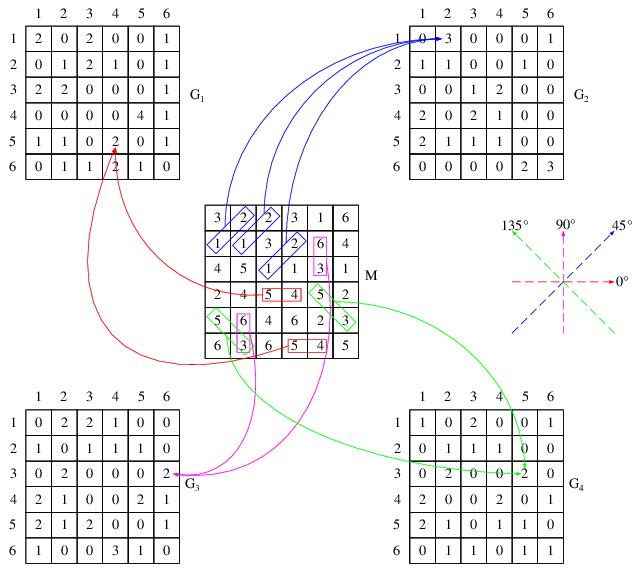
\includegraphics[width=8cm,height=8cm,keepaspectratio]{glcm.png}
    \end{figure}

    
    \setlength{\baselineskip}{0.8cm}
    {\vspace{0.5cm}\fontsize{6mm}{6mm}\selectfont Successivamente attraverso la funzione graycoprops normalizziamo i valori presenti nella glcm cosicchè la somma dei valori presenti al suo interno sia uguale ad 1, specificando come secondo parametro della funzione la proprietà 'contrast', la quale restituisce il valore dell'intensità del contrasto tra un pixel e quello a lui adiacente. In questa maniera otteniamo i valori e le posizioni dei pixel che si ripetono di più all'interno dell'immagine e con la funzione 'plot' andiamo a rappresentarle graficamente. Dopodichè, filtrando in maniera opportuna i valori massimi, selezioniamo il valore ideale con il quale creare i nostri pattern.}
    
    \vspace{0.5cm}
    
    \begin{figure}[H]
        \centering
        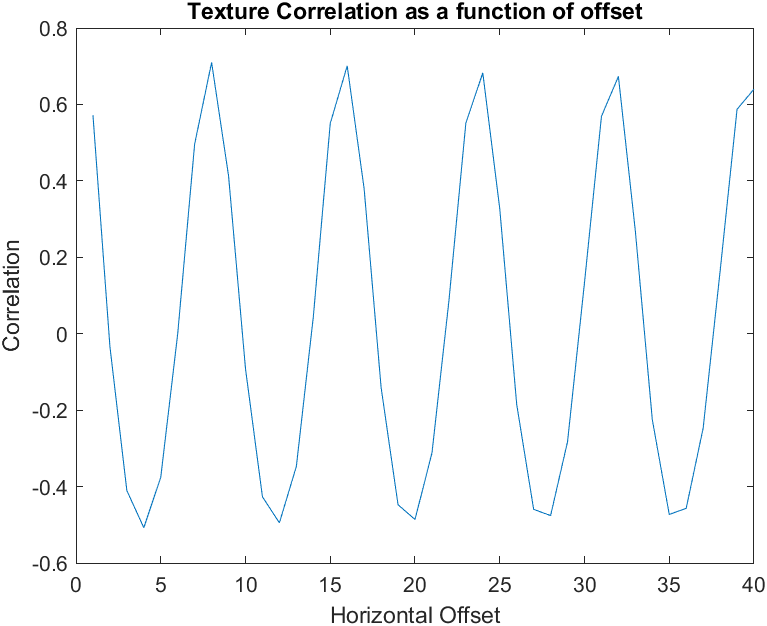
\includegraphics[width=8cm,height=8cm,keepaspectratio]{Grafico_massimi_ESI.png}
    \end{figure}
    
   \vspace{0.5cm}
   
    \subsection{Cross Correlazione}
    
    \setlength{\baselineskip}{0.8cm}
    {\vspace{0.5cm}\fontsize{6mm}{6mm}\selectfont Dopo aver ottenuto 10 pattern di dimensione ideale abbiamo calcolato la cross correlazione tra questi ultimi e l'immagine originale ottenendo 10 matrici, dalle quali abbiamo poi ricavato la matrice media. La media dei valori all'interno di essa verrà confrontata con il valore di 0.07 (ottenuto mediante un procedimento euristico ed osservando i vari valori che si ottenevano dalle diverse immagini) con lo scopo di scegliere il raggio da utilizzare nella funzione 'strel'. }
    

    \subsection{Graythreshold}
    
    
    \setlength{\baselineskip}{0.8cm}
    {\vspace{0.5cm}\fontsize{6mm}{6mm}\selectfont Con la funzione 'graythresh' otteniamo una treshold, mediante l'utilizzo del metodo di Otsu, dall'immagine ottenuta in precendeza attraverso la cross correlazione per poi costruire una maschera che rende neri i pixel che hanno un valore maggiore della graytreshold e bianchi i pixel che hanno un valore minore della treshold.  }
    
    
    \begin{figure}[H]
        \centering
        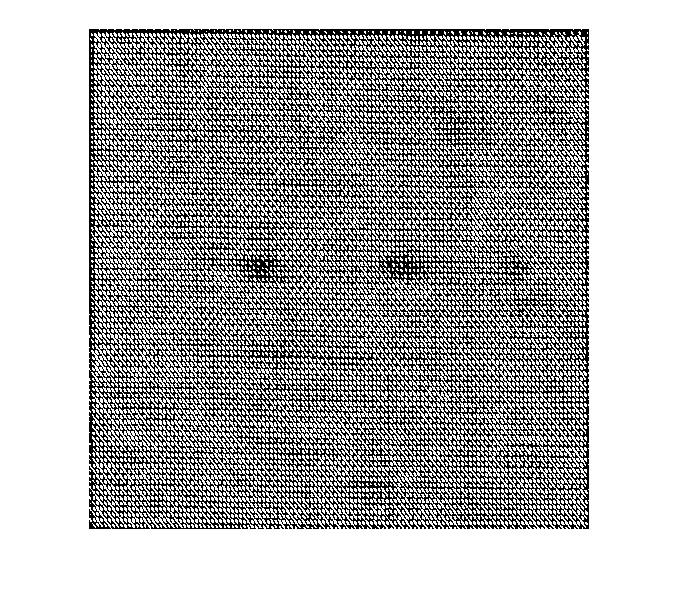
\includegraphics[width=8cm,height=8cm,keepaspectratio]{graythreshold.jpg}
    \end{figure}
    
    
    \subsection{Elaborazione della maschera}
    
    \setlength{\baselineskip}{0.8cm}
    {\vspace{0.5cm}\fontsize{6mm}{6mm}\selectfont Dopo aver ottenuto la maschera dal passo precedente iniziamo l'elaborazione mediante la funzione 'strel' con l'aggiunta del parametro 'disk' la quale ci permette di valutare i valori binari di un determinato intorno discoidale di un pixel mantenendo solamente quelli ad 1 e scartando quelli a 0, ciò permetterà di prendere in considerazione solamente le parti del difetto della tessitura che sono state trovate nella fase precedente. Successivamente utilizziamo la funzione 'imdilate' per evidenziare in maniera più marcata quelle zone della matrice che corrispondono al difetto. Inoltre con la funzione 'imcomplement' invertiamo i valori dei pixel della maschera in quanto ci permetterà di evidenziare nell'immagine originale i pixel che corrispondono al difetto. Mediante la funzione 'bwconncomp' calcoliamo il numero di componenti connesse ed andremo ad utilizzarlo nella funzione 'bwareafilt' la quale ritornerà una nuova maschera in cui sono evidenziate solamente le le aree che corrspondono ai difetti dell'immagine.}
    
    \begin{figure}[H]
        \centering
        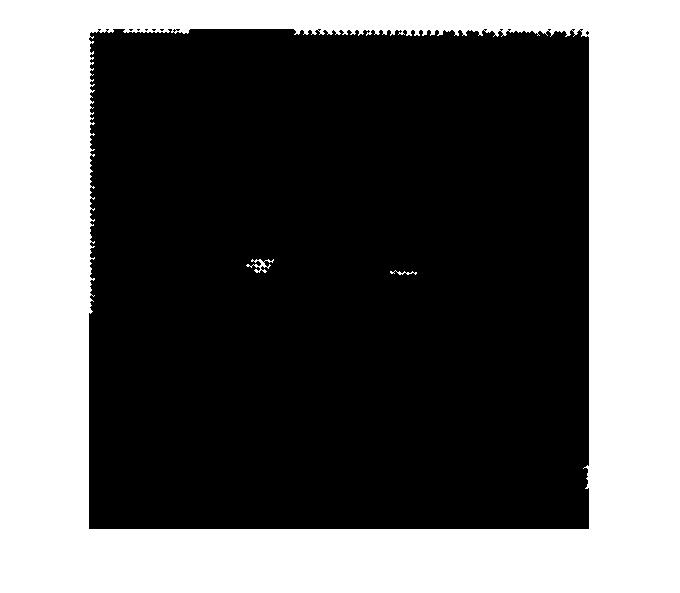
\includegraphics[width=8cm,height=8cm,keepaspectratio]{maschera_terminata.jpg}
    \end{figure}
    
    
    \vspace{0.5cm}
    \subsection{Applicazione della maschera}
    
    \setlength{\baselineskip}{0.8cm}
    {\vspace{0.5cm}\fontsize{6mm}{6mm}\selectfont Per concludere abbiamo ritagliato il perimetro dell'immagine originale in modo che sia della dimensione di 500x500 e mediante la maschera ottenuta con i passaggi precedenti abbiamo dato ai pixel che corrispondono al difetto di tessitura il valore di 255 in maniera tale che siano evidenziati in rosso nella figura iniziale. }
    
    \begin{figure}[H]
        \centering
        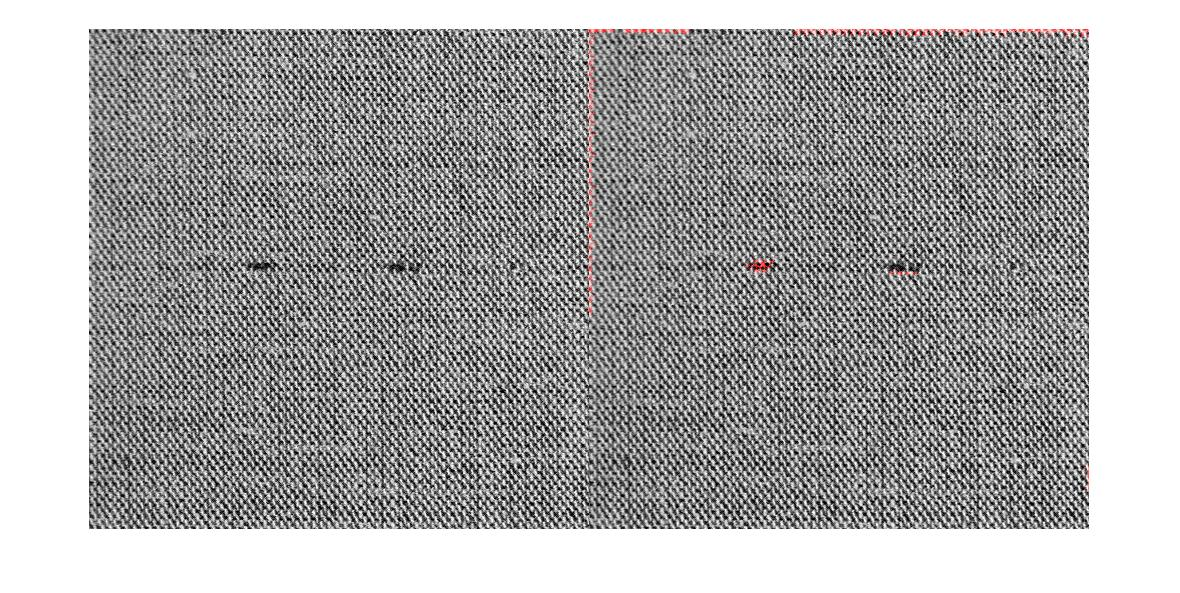
\includegraphics[width=15cm,height=15cm,keepaspectratio]{risultato_finale.jpg}
    \end{figure}

    
\vspace{0.5cm}
\section{Conclusioni}
\setlength{\baselineskip}{0.8cm}
    {\vspace{0.5cm}\fontsize{6mm}{6mm}\selectfont Come risultato finale abbiamo ottenuto un programma Matlab che ci permette di rilevare in maniera automatica ,cioè senza dover modificare manualmente i vari parametri che regolano l'evidenziazione dell'errore, i vari difetti delle tessiture che vengono dati in input. Ovviamente è necessario che le immagini elaborate dal programma siano di una certa dimensione (512px x 512px) per essere elaborate in maniera ottimale. E' necessario rendere noto inoltre che nel caso in cui il difetto sia troppo simile al pattern di pixel presente su tutta l'immagine lo script farà fatica a rilevare l'errore questo a causa dell'approccio da noi adottato, però supponiamo che un campione simile sia statisticamente più difficile da trovare rispetto alla media dei casi. }

\end{document}